\documentclass[12pt]{article}
\usepackage{colortbl}
\usepackage{booktabs}
\usepackage{tikz}
\usetikzlibrary{bayesnet}

\input{cs486_assign_preamble.tex}

\lhead{CS 486/686}
\chead{Spring 2024}
\rhead{Assignment 1}
\cfoot{v1.0}
\lfoot{\copyright Wenhu Chen 2024}

\title{CS 486/686 Assignment 1 \\ Spring 2024 \\ (100 marks) }
\author{Instructor: Wenhu Chen}
\date{Due Date: 11:59PM on Jun 13rd}

\newcommand\independent{\perp\!\!\!\perp}

\begin{document}

\maketitle

\section*{Instructions}

\begin{itemize}
	\item Submit your written answers and ipynb as two separate files to LEARN. The written answers need to be submitted as a PDF.

	\item
	      No late assignment will be accepted. This assignment is to be done individually.

	\item
	      Lead TAs:
	      \begin{itemize}
		      \item
		            Yongdong Luo (\url{yudong.luo@uwaterloo.ca})
		      \item
		            Aref Jafari (\url{aref.jafari@uwaterloo.ca})
		      \item
		            Rui ming Xiong (\url{rmxiong@uwaterloo.ca})
	      \end{itemize}
	      The TAs' office hours will be scheduled and posted on LEARN and Piazza.
\end{itemize}

\section*{Learning Goal}
\begin{itemize}
	\item Learning to determine the unconditional and conditional dependence between variables from the joint probability distribution.
	\item Learning to construct Bayesian network and how to encode Bayesian network.
	\item Learning to how to do backward propagation.
	\item Implementing different optimization strategies in neural networks.
\end{itemize}


\section{Reconstructing Bayesian Network (30 marks)}
Given four boolean random variables A, B, C, D, there are some underlying (conditional) independence between these variables. You are supposed to identify these (conditional) independence between variables, and then reconstruct the \textbf{most compact Bayesian Network} (minimum number probabilities to encode the network). The joint probability distribution is in Table~\ref{tab:joint_distribution}.

\begin{table}[!h]
	\centering
	\begin{tabular}{llllc}
		\toprule
		A & B & C & D & Prob   \\
		\midrule
		T & T & T & T & 0.0080 \\
		T & T & T & F & 0.0120 \\
		T & T & F & T & 0.0080 \\
		T & T & F & F & 0.0120 \\
		T & F & T & T & 0.0576 \\
		T & F & T & F & 0.0144 \\
		T & F & F & T & 0.1344 \\
		T & F & F & F & 0.0336 \\
		F & T & T & T & 0.1080 \\
		F & T & T & F & 0.0720 \\
		F & T & F & T & 0.0720 \\
		F & T & F & F & 0.1080 \\
		F & F & T & T & 0.0864 \\
		F & F & T & F & 0.0216 \\
		F & F & F & T & 0.2016 \\
		F & F & F & F & 0.0504 \\
		\bottomrule
		\hline
	\end{tabular}
	\caption{Joint probability distribution of $P(A, B, C, D)$.}
	\arrayrulecolor{black}
	\label{tab:joint_distribution}
\end{table}

\begin{enumerate}[font=\Large,label=(\alph*)]
	\item Is variable A independent from variable D?
	      $$
		      \begin{array}{|c|c|}
			      \hline
			      A & P(A)                                                         \\
			      \hline
			      T & 0.0080+0.0120+0.0080+0.0120+0.0576+0.0144+0.1344+0.0336=0.28 \\
			      F & 0.0720+0.1080+0.0720+0.1080+0.0864+0.0216+0.2016+0.0504=0.72 \\
			      \hline
		      \end{array}
	      $$
	      $$
		      \begin{array}{|c|c|}
			      \hline
			      D & P(D)                                                          \\
			      \hline
			      T & 0.0080+0.0080+0.0576+0.1344+0.1080+0.0720+0.0864+0.2016=0.676 \\
			      F & 0.0120+0.0120+0.0144+0.0336+0.0720+0.1080+0.0216+0.0504=0.324 \\
			      \hline
		      \end{array}
	      $$

	      Joint Probability Table for $ P(A, D) $:

	      $$
		      \begin{array}{|c|c|c|c|}
			      \hline
			      A & D & P(A, D)                           & P(A)\cdot P(D) \\
			      \hline
			      T & T & 0.0080+0.0080+0.0576+0.1344=0.208 & 0.18928        \\
			      T & F & 0.0120+0.0120+0.0144+0.0336=0.072 & 0.09072        \\
			      F & T & 0.1080+0.0720+0.0864+0.2016=0.468 & 0.48672        \\
			      F & F & 0.0720+0.1080+0.0216+0.0504=0.252 & 0.23328        \\
			      \hline
		      \end{array}
	      $$

	      $ P(A, D) \neq P(A) P(D) $ for all $A,D$. Therefore, variable A is not independent from variable D.

	\item Given A, are the random variable C and D independent from each other?

	      $$ P(A = T, C = T) = 0.0080 + 0.0120 + 0.0576 + 0.0144 = 0.092 $$
	      $$ P(A = T, C = F) = 0.0080 + 0.0120 + 0.1344 + 0.0336 = 0.188 $$
	      $$ P(A = F, C = T) = 0.0720 + 0.1080 + 0.0864 + 0.0216 = 0.288 $$
	      $$ P(A = F, C = F) = 0.0720 + 0.1080 + 0.2016 + 0.0504 = 0.432 $$
	      $$
		      \begin{array}{|c|c|c|}
			      \hline
			      (A) & C & P(C \mid A)       \\
			      \hline
			      T   & T & 0.092/0.28=0.3286 \\
			      T   & F & 0.188/0.28=0.6714 \\
			      \hline
			      F   & T & 0.288/0.72=0.4    \\
			      F   & F & 0.432/0.72=0.6    \\
			      \hline
		      \end{array}
	      $$
	      $$
		      \begin{array}{|c|c|c|}
			      \hline
			      (A) & D & P(D \mid A)       \\
			      \hline
			      T   & T & 0.208/0.28=0.7429 \\
			      T   & F & 0.072/0.28=0.2571 \\
			      \hline
			      F   & T & 0.468/0.72=0.65   \\
			      F   & F & 0.252/0.72=0.35   \\
			      \hline
		      \end{array}
	      $$

	      Compare $ P(C, D \mid A) $ with $ P(C \mid A) \cdot P(D \mid A) $:

	      $$
		      \begin{array}{|c|c|c|c|c|}
			      \hline
			      (A) & C & D & P(C, D \mid A)                & P(C \mid A) \cdot P(D \mid A) \\
			      \hline
			      T   & T & T & (0.008+0.0576)/0.28 = 0.2343  & 0.3286 \times 0.7429 = 0.2441 \\
			      T   & T & F & (0.012+0.0144)/0.28 = 0.0943  & 0.3286 \times 0.2571 = 0.0845 \\
			      T   & F & T & (0.0080+0.1344)/0.28 = 0.5086 & 0.6714 \times 0.7429 = 0.4988 \\
			      T   & F & F & (0.0120+0.0336)/0.28 = 0.1629 & 0.6714 \times 0.2571 = 0.1726 \\
			      \hline
			      F   & T & T & (0.108+0.0864)/0.72 = 0.27    & 0.4 \times 0.65 = 0.26        \\
			      F   & T & F & (0.0216+0.072)/0.72 = 0.13    & 0.4 \times 0.35 = 0.14        \\
			      F   & F & T & (0.0720+0.2016)/0.72 = 0.38   & 0.6 \times 0.65 = 0.39        \\
			      F   & F & F & (0.1080+0.0504)/0.72 = 0.22   & 0.6 \times 0.35 = 0.21        \\
			      \hline
		      \end{array}
	      $$

	      $ P(C, D \mid A) \neq P(C \mid A) \cdot P(D \mid A) $ for all combinations of $A,C,D$. Therefore, C and D are not conditionally independent given A.
	      \newpage
	\item Given B, is the random variable A independent from C?
	      $$ P(B = T) = 0.0080 + 0.0120 + 0.0080 + 0.0120 + 0.1080 + 0.0720 + 0.0720 + 0.1080 = 0.4 $$
	      $$ P(B = F) = 0.0576 + 0.0144 + 0.1344 + 0.0336 + 0.0864 + 0.0216 + 0.2016 + 0.0504 = 0.6 $$

	      $$
		      \begin{array}{|c|c|c|}
			      \hline
			      (B) & A & P(A \mid B)                                 \\
			      \hline
			      T   & T & (0.0080+0.0120+0.0080+0.0120)/0.4=0.1       \\
			      T   & F & (0.1080 + 0.0720 + 0.0720 + 0.1080)/0.4=0.9 \\
			      F   & T & (0.0576 + 0.0144 + 0.1344 + 0.0336)/0.6=0.4 \\
			      F   & F & (0.0864 + 0.0216 + 0.2016 + 0.0504)/0.6=0.6 \\
			      \hline
		      \end{array}
	      $$

	      $$
		      \begin{array}{|c|c|c|}
			      \hline
			      (B) & C & P(C \mid B)                               \\
			      \hline
			      T   & T & (0.0080 + 0.0120+0.1080 + 0.0720)/0.4=0.5 \\
			      T   & F & (0.0080 + 0.0120+0.1080 + 0.0720)/0.4=0.5 \\
			      F   & T & (0.0576 + 0.0144+0.0864 + 0.0216)/0.6=0.3 \\
			      F   & F & (0.1344 + 0.0336+0.2016 + 0.0504)/0.6=0.7 \\
			      \hline
		      \end{array}
	      $$

	      $ P(A, C \mid B) $ vs $ P(A \mid B) \cdot P(C \mid B) $:

	      $$
		      \begin{array}{|c|c|c|c|c|}
			      \hline
			      (B) & A & C & P(A, C \mid B)           & P(A \mid B) \cdot P(C \mid B) \\
			      \hline
			      T   & T & T & (0.0080+0.0120)/0.4=0.05 & 0.1 \times 0.5 = 0.05         \\
			      T   & T & F & (0.0080+0.0120)/0.4=0.05 & 0.1 \times 0.5 = 0.05         \\
			      T   & F & T & (0.0720+0.1080)/0.4=0.45 & 0.9 \times 0.5 = 0.45         \\
			      T   & F & F & (0.0720+0.1080)/0.4=0.45 & 0.9 \times 0.5 = 0.45         \\
			      \hline
			      F   & T & T & (0.0576+0.0144)/0.6=0.12 & 0.4 \times 0.3 = 0.12         \\
			      F   & T & F & (0.1344+0.0336)/0.6=0.28 & 0.4 \times 0.7 = 0.28         \\
			      F   & F & T & (0.0864+0.0216)/0.6=0.18 & 0.6 \times 0.3 = 0.18         \\
			      F   & F & F & (0.2016+0.0504)/0.6=0.42 & 0.6 \times 0.7 = 0.42         \\
			      \hline
		      \end{array}
	      $$

	      $P(A, C \mid B) = P(A \mid B) \cdot P(C \mid B)$ for all combinations of $A,B,C$. Therefore, the random variable $A$ is independent from $C$ given $B$.

	\item Given B, is the random variable A independent from D?
	      $$
		      \begin{array}{|c|c|c|}
			      \hline
			      (B) & D & P(D \mid B)                                  \\
			      \hline
			      T   & T & (0.0080 + 0.0080 + 0.1080 + 0.0720)/0.4=0.49 \\
			      T   & F & (0.0120 + 0.0120 + 0.0720 + 0.1080)/0.4=0.51 \\
			      F   & T & (0.0576 + 0.1344 + 0.0864 + 0.2016)/0.6=0.8  \\
			      F   & F & (0.0144 + 0.0336 + 0.0216 + 0.0504)/0.6=0.2  \\
			      \hline
		      \end{array}
	      $$

	      $P(A, D \mid B)$ vs $P(A \mid B) \cdot P(D \mid B):$

	      $$
		      \begin{array}{|c|c|c|c|c|}
			      \hline
			      (B) & A & D & P(A, D \mid B)               & P(A \mid B) \cdot P(D \mid B) \\
			      \hline
			      T   & T & T & (0.0080 + 0.0080)/0.4 = 0.04 & 0.1 \times 0.49 = 0.049       \\
			      T   & T & F & (0.0120 + 0.0120)/0.4 = 0.06 & 0.1 \times 0.51 = 0.051       \\
			      T   & F & T & (0.1080 + 0.0720)/0.4 = 0.45 & 0.9 \times 0.49 = 0.441       \\
			      T   & F & F & (0.0720 + 0.1080)/0.4 = 0.45 & 0.9 \times 0.51 = 0.459       \\
			      \hline
			      F   & T & T & (0.0576 + 0.1344)/0.6 = 0.32 & 0.4 \times 0.8 = 0.32         \\
			      F   & T & F & (0.0144 + 0.0336)/0.6 = 0.08 & 0.4 \times 0.2 = 0.08         \\
			      F   & F & T & (0.0864 + 0.2016)/0.6 = 0.48 & 0.6 \times 0.8 = 0.48         \\
			      F   & F & F & (0.0216 + 0.0504)/0.6 = 0.12 & 0.6 \times 0.2 = 0.12         \\
			      \hline
		      \end{array}
	      $$

	      $P(A, D \mid B) \neq P(A \mid B) \cdot P(D \mid B)$ for all combinations of $A,D$ given $B=T$. Therefore, the random variable $A$ is not independent from $D$ given $B$.

	\item Given B, is the random variable C independent from D?

	      $$
		      \begin{array}{|c|c|c|}
			      \hline
			      (B) & C & P(C \mid B) \\
			      \hline
			      T   & T & 0.2/0.4=0.5 \\
			      T   & F & 0.2/0.4=0.5 \\
			      F   & T & 1.8/0.6=0.3 \\
			      F   & F & 4.2/0.6=0.7 \\
			      \hline
		      \end{array}
	      $$

	      $P(C, D \mid B)$ vs $P(C \mid B) \cdot P(D \mid B):$

	      $$
		      \begin{array}{|c|c|c|c|c|}
			      \hline
			      (B) & C & D & P(C, D \mid B)   & P(C \mid B) \cdot P(D \mid B) \\
			      \hline
			      T   & T & T & 0.116/0.4 = 0.29 & 0.5 \times 0.49 = 0.245       \\
			      T   & T & F & 0.084/0.4 = 0.21 & 0.5 \times 0.51 = 0.255       \\
			      T   & F & T & 0.080/0.4 = 0.2  & 0.5 \times 0.49 = 0.245       \\
			      T   & F & F & 0.120/0.4 = 0.3  & 0.5 \times 0.51 = 0.255       \\
			      \hline
			      F   & T & T & 0.144/0.6 = 0.24 & 0.3 \times 0.8 = 0.24         \\
			      F   & T & F & 0.036/0.6 = 0.06 & 0.3 \times 0.2 = 0.06         \\
			      F   & F & T & 0.336/0.6 = 0.56 & 0.7 \times 0.8 = 0.56         \\
			      F   & F & F & 0.084/0.6 = 0.14 & 0.7 \times 0.2 = 0.14         \\
			      \hline
		      \end{array}
	      $$

	      $P(C, D \mid B) \neq P(C \mid B) \cdot P(D \mid B)$ for all combinations of $C,D$ given $B=T$. Therefore, the random variable $C$ is not independent from $D$ given $B$.

	      \newpage
	\item Show the Bayesian Network if we construct it in the order of B, A, C, D. How many probabilities do we need to represent this constructed Bayesian Network?
	      \begin{center}
		      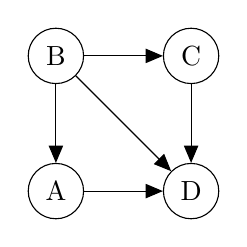
\begin{tikzpicture}
			      % Define nodes
			      \node[latent] (B) {B};
			      \node[latent, below=of B] (A) {A};
			      \node[latent, right=of B] (C) {C};
			      \node[latent, right=of A] (D) {D};

			      % Connect the nodes
			      \edge {B} {A};
			      \edge {B} {C};
			      \edge {A, B, C} {D};
		      \end{tikzpicture}
	      \end{center}

	      Probabilities Needed:\\
	      - $ P(B) $: 1 probability\\
	      - $ P(A \mid B) $: 2 probabilities\\
	      - $ P(C \mid B) $: 2 probabilities\\
	      - $ P(D \mid A, B, C) $: 8 probabilities

	      Total: $ 1 + 2 + 2 + 8 = 13 $ probabilities

	\item Show the Bayesian Network if we construct it in the order of A, C, B, D. How many probabilities do we need to represent this constructed Bayesian Network?
	      \begin{center}
		      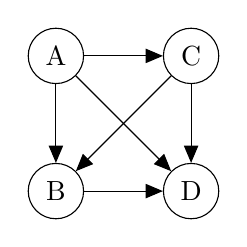
\begin{tikzpicture}
			      % Define nodes
			      \node[latent] (A) {A};
			      \node[latent, right=of A] (C) {C};
			      \node[latent, below=of A] (B) {B};
			      \node[latent, right=of B] (D) {D};

			      % Connect the nodes
			      \edge {A} {C};
			      \edge {A, C} {B};
			      \edge {A, B, C} {D};
		      \end{tikzpicture}
	      \end{center}

	      Probabilities Needed:

	      - $ P(A) $: 1 probability

	      - $ P(C \mid A) $: 2 probabilities

	      - $ P(B \mid A, C) $: 4 probabilities

	      - $ P(D \mid A, B, C) $: 8 probabilities

	      Total: $ 1 + 2 + 4 + 8 = 15 $ probabilities

	\item We have already derived two Bayesian Networks so far based on the given order. Are they the most compact Bayesian Networks, i.e., having the smallest amount of probabilities? Is there any other Bayesian Network that is most compact?

	      The Bayesian Net in (f) is the most compact but in (g) is not

	      There exists other most compact Bayesian Net e.g. A, B, C, D
\end{enumerate}

\newpage
\section{Backward propagation (35 marks)}
Skip connections, also known as residual connections, are standard components in many deep neural network architectures. In these connections, the outputs of preceding layers are summed with later layers. This provides an alternative pathway for gradients during backpropagation, which has been shown to significantly enhance model convergence and help prevent the vanishing gradient problem. For the summation to be possible in skip connections, the dimensions of the layers involved must be similar.
\begin{figure*}[hbt]
	\centering
	\includegraphics[width=0.8\textwidth]{skip_connection.png}
	\caption{A simple 2-layer neural network with skip connection. }
	\label{fig:pipeline}
\end{figure*}


In this question, we consider a modified version of the simple 2-layer neural network from the course notes, which was used for binary classification of emails as spam or not spam. The network is redefined to include skip connections. Figure 1 illustrates the modified network, where the green connections represent the skip connections. For simplicity, biases have been removed.

\begin{equation}
	a^{(1)}_j = \sum_i x_i W_{i,j}^{(1)}\qquad,\qquad z_j^{(1)} = g(a^{(1)}_j) + x_j
\end{equation}

\begin{equation}
	a^{(2)}_k = \sum_j z_j^{(1)} W_{j,k}^{(2)}\qquad,\qquad z_k^{(2)} = g(a^{(2)}_k) + z_k^{(1)}
\end{equation}

The input features are $x_1$ (email length) and $x_2$ (whether the email is from a trusted organization). The output is a binary classification with $z^{(2)}_1$ indicating the likelihood of being spam and $z^{(2)}_2$ indicating the likelihood of not being spam.

* \textbf{Note:} You can do all your calculations in matrix form.

\begin{equation}
	\textbf{a}^{(1)} = \textbf{x} W^{(1)}\qquad,\qquad \textbf{z}^{(1)} = g(\textbf{a}^{(1)}) + \textbf{x}
\end{equation}

\begin{equation}
	\textbf{a}^{(2)} = \textbf{z}^{(1)} W^{(2)}\qquad,\qquad \textbf{z}^{(2)} = g(\textbf{a}^{(2)}) + \textbf{z}^{(1)}
\end{equation}

Where $W^{(1)}, W^{(2)} \in R^{2\times 2}$ and $\textbf{a}^{(1)}, \textbf{a}^{(2)}, \textbf{z}^{(1)}, \textbf{z}^{(2)} \in R^2$, and g is an activation function.

\begin{enumerate}[font=\Large]
	\item \textbf{Forward Pass: (5 marks)}\\
	      Given the following weights for the network:
	      $$
		      W^{(1)} = \begin{bmatrix}
			      0.2 & -0.3 \\
			      0.4 & 0.1
		      \end{bmatrix}, \quad
		      W^{(2)} = \begin{bmatrix}
			      0.7  & 0.5 \\
			      -0.6 & 0.2
		      \end{bmatrix}, \quad
	      $$

	      Compute the output of the network for an input $x=[0.5,1.0]$ using the sigmoid ($\frac{1}{1+e^{-x}}$) activation function.
	      $$
		      \mathbf{a}^{(1)} = \mathbf{x} W^{(1)} = \begin{bmatrix} 0.5 & 1.0 \end{bmatrix} \begin{bmatrix} 0.2 & -0.3 \\ 0.4 & 0.1 \end{bmatrix} = \begin{bmatrix} 0.5 & -0.05 \end{bmatrix}
	      $$
	      $$
		      g(\mathbf{a}^{(1)}) = \begin{bmatrix} \dfrac{1}{1 + e^{-0.5}} & \dfrac{1}{1 + e^{0.05}} \end{bmatrix} \approx \begin{bmatrix} 0.6225 & 0.4875 \end{bmatrix}
	      $$
	      $$
		      \mathbf{z}^{(1)} = g(\mathbf{a}^{(1)}) + \mathbf{x} \approx \begin{bmatrix} 0.6225 & 0.4875 \end{bmatrix} + \begin{bmatrix} 0.5 & 1.0 \end{bmatrix} = \begin{bmatrix} 1.1225 & 1.4875 \end{bmatrix}
	      $$
	      $$
		      \mathbf{a}^{(2)} = \mathbf{z}^{(1)} W^{(2)} \approx \begin{bmatrix} 1.1225 & 1.4875 \end{bmatrix} \begin{bmatrix} 0.7 & 0.5 \\ -0.6 & 0.2 \end{bmatrix} = \begin{bmatrix} -0.1068 & 0.8588 \end{bmatrix}
	      $$
	      $$
		      g(\mathbf{a}^{(2)}) = \begin{bmatrix} \dfrac{1}{1 + e^{0.1068}} & \dfrac{1}{1 + e^{-0.8588}} \end{bmatrix} \approx \begin{bmatrix} 0.4733 & 0.7024 \end{bmatrix}
	      $$
	      $$
		      \mathbf{z}^{(2)} = g(\mathbf{a}^{(2)}) + \mathbf{z}^{(1)} \approx \begin{bmatrix} 0.4733 & 0.7024 \end{bmatrix} + \begin{bmatrix} 1.1225 & 1.4875 \end{bmatrix} = \begin{bmatrix} 1.5958 & 2.1899 \end{bmatrix}
	      $$

	\item \textbf{Error Calculation: (5 marks)} \\
	      If the true label for the given input is $y=[1,0]$, compute the loss using the sum of squares error function.
	      $$
		      L = \sum_{k=1}^2 (z_k^{(2)} - y_k)^2 \approx (1.5958 - 1)^2+(2.1899 - 0)^2 = 5.1506
	      $$
	      \newpage
	\item \textbf{Backward Pass: (8 marks)}\\
	      Derive the gradients of the error with respect to the weights $W^{(2)}$ and $W^{(1)}$ using backpropagation. Show all steps clearly.
	      $$g'(\mathbf{a}^{(2)})=\begin{bmatrix} 0.4733(1-0.4733) & 0.7024(1-0.7024) \end{bmatrix}=\begin{bmatrix} 0.2493 & 0.2090 \end{bmatrix}$$
	      $$g'(\mathbf{a}^{(1)})=\begin{bmatrix} 0.6225(1-0.6225) &  0.4875(1- 0.4875) \end{bmatrix}=\begin{bmatrix} 0.2350 & 0.2498 \end{bmatrix}$$
	      $$
		      \begin{aligned}
			      \delta_2= & \dfrac{\partial L}{\partial z^{(2)}} g'(\mathbf{a}^{(2)})                                                                          \\
			      =         & 2(\begin{bmatrix} 1.5958 & 2.1899 \end{bmatrix}-\begin{bmatrix} 1 & 0 \end{bmatrix}) \begin{bmatrix} 0.2493 & 0.2090 \end{bmatrix} \\
			      =         & \begin{bmatrix} 0.2970 & 0.9155 \end{bmatrix}
		      \end{aligned}$$
	      $$
		      \begin{aligned}
			      \delta_1= & \delta_2\cdot W_2^T\cdot g'(\mathbf{a}^{(1)})                                                                                                \\
			      =         & \begin{bmatrix} 0.2970 & 0.9155 \end{bmatrix}\begin{bmatrix}0.7 & -0.6 \\0.5 & 0.2\end{bmatrix}\begin{bmatrix} 0.2350 & 0.2498 \end{bmatrix} \\
			      =         & \begin{bmatrix} 0.1564 & 0.0012 \end{bmatrix}
		      \end{aligned}
	      $$
	      $$\dfrac{\partial L}{\partial W^{(2)}}=\delta_2\otimes\mathbf{z}^{(1)}=\begin{bmatrix} 1.1225 \\ 1.4875 \end{bmatrix}\begin{bmatrix} 0.2970 & 0.9155 \end{bmatrix}=\begin{bmatrix} 0.3334 & 1.0276\\ 0.4418 & 1.3618 \end{bmatrix}$$
	      $$\dfrac{\partial L}{\partial W^{(1)}}=\delta_1\otimes\mathbf{x}=\begin{bmatrix} 0.5 \\ 1 \end{bmatrix}\begin{bmatrix} 0.1564 & 0.0012 \end{bmatrix}=\begin{bmatrix} 0.0782 & 0.0006\\ 0.1564 & 0.0012 \end{bmatrix}$$
	\item \textbf{Weight Update: (5 marks)}\\
	      Using a learning rate $\eta=0.1$, update the weights $W^{(2)}$ and $W^{(1)}$. Provide the updated weights.
	      $$W^{(1)}=W^{(1)}-\eta\dfrac{\partial L}{\partial W^{(1)}}=\begin{bmatrix}
			      0.2 & -0.3 \\
			      0.4 & 0.1
		      \end{bmatrix}
		      -0.1\begin{bmatrix} 0.0782 & 0.0006\\ 0.1564 & 0.0012 \end{bmatrix}=\begin{bmatrix} 0.1922 & 0.30006\\ 0.3844 & 0.09998 \end{bmatrix}$$
	      $$W^{(2)}=W^{(2)}-\eta\dfrac{\partial L}{\partial W^{(2)}}= \begin{bmatrix}
			      0.7  & 0.5 \\
			      -0.6 & 0.2
		      \end{bmatrix}-0.1\begin{bmatrix} 0.3334 & 1.0276\\ 0.4418 & 1.3618 \end{bmatrix}=\begin{bmatrix} 0.66666 & 0.39724\\ -0.64418 & 0.06382 \end{bmatrix}$$

	      \newpage
	\item \textbf{Different Activation: (4 marks)}\\
	      Derive the gradients of the error with respect to the weights $W^{(2)}$ and $W^{(1)}$ using backpropagation, but with a new activation function ReLU for both layers, i.e. $max(x, 0)$. Show all steps clearly.
	      $$
		      \mathbf{a}^{(1)} = \mathbf{x} W^{(1)} = \begin{bmatrix} 0.5 & 1.0 \end{bmatrix} \begin{bmatrix} 0.2 & -0.3 \\ 0.4 & 0.1 \end{bmatrix} = \begin{bmatrix} 0.5 & -0.05 \end{bmatrix}
	      $$
	      $$
		      g(\mathbf{a}^{(1)}) =  \begin{bmatrix} 0.5 & 0 \end{bmatrix}
	      $$
	      $$
		      \mathbf{z}^{(1)} = g(\mathbf{a}^{(1)}) + \mathbf{x} = \begin{bmatrix} 0.5 & 0 \end{bmatrix} + \begin{bmatrix} 0.5 & 1.0 \end{bmatrix} = \begin{bmatrix} 1 & 1 \end{bmatrix}
	      $$
	      $$
		      \mathbf{a}^{(2)} = \mathbf{z}^{(1)} W^{(2)} = \begin{bmatrix} 1 & 1 \end{bmatrix} \begin{bmatrix} 0.7 & 0.5 \\ -0.6 & 0.2 \end{bmatrix} = \begin{bmatrix} 0.1 & 0.7 \end{bmatrix}
	      $$
	      $$
		      g(\mathbf{a}^{(2)}) = \begin{bmatrix} 0.1 & 0.7 \end{bmatrix}
	      $$
	      $$
		      \mathbf{z}^{(2)} = g(\mathbf{a}^{(2)}) + \mathbf{z}^{(1)} =\begin{bmatrix} 0.1 & 0.7 \end{bmatrix} + \begin{bmatrix} 1 & 1 \end{bmatrix} = \begin{bmatrix} 1.1 & 1.7 \end{bmatrix}
	      $$
	      $$g'(\mathbf{a}^{(1)})=\begin{bmatrix} 1 & 0 \end{bmatrix}$$
	      $$g'(\mathbf{a}^{(2)})=\begin{bmatrix} 1 & 1 \end{bmatrix}$$
	      $$
		      \begin{aligned}
			      \delta_2= & \dfrac{\partial L}{\partial \textbf{z}^{(2)}} g'(\mathbf{a}^{(2)})                                                 \\
			      =         & 2(\begin{bmatrix} 1.1 & 1.7 \end{bmatrix}-\begin{bmatrix} 1 & 1 \end{bmatrix}) \begin{bmatrix} 1 & 1 \end{bmatrix} \\
			      =         & \begin{bmatrix} 0.2 & 1.4 \end{bmatrix}
		      \end{aligned}$$
	      $$
		      \begin{aligned}
			      \delta_1= & \delta_2\cdot W_2^T\cdot g'(\mathbf{a}^{(1)})                                                                                \\
			      =         & \begin{bmatrix} 0.2 & 1.4 \end{bmatrix}\begin{bmatrix}0.7 & -0.6 \\0.5 & 0.2\end{bmatrix}\begin{bmatrix} 1 & 0 \end{bmatrix} \\
			      =         & \begin{bmatrix} 0.84 & 0 \end{bmatrix}
		      \end{aligned}
	      $$
	      $$\dfrac{\partial L}{\partial W^{(2)}}=\delta_2\otimes\mathbf{z}^{(1)}=\begin{bmatrix} 1 \\ 1 \end{bmatrix}\begin{bmatrix} 0.2 & 1.4 \end{bmatrix}=\begin{bmatrix} 0.2 & 1.4\\ 0.2 & 1.4 \end{bmatrix}$$
	      $$\dfrac{\partial L}{\partial W^{(1)}}=\delta_1\otimes\mathbf{x}=\begin{bmatrix} 0.5 \\ 1 \end{bmatrix}\begin{bmatrix} 0.84 & 0 \end{bmatrix}=\begin{bmatrix} 0.42 & 0\\ 0.84 & 0 \end{bmatrix}$$

	      \newpage
	\item \textbf{Practical Considerations: (8 marks)}
	      \begin{enumerate}[label=(\alph*)]
		      \item (4 marks) Discuss the impact of learning rate on the convergence of the backpropagation algorithm. What are the potential issues with choosing a very high or very low learning rate?
		            \begin{itemize}
			            \item High Learning Rate
			                  \begin{itemize}
				                  \item Pros: A higher learning rate can speed up the convergence process because it takes larger steps towards the minimum of the loss function.
				                  \item Cons: If the learning rate is too high, the algorithm might overshoot the minimum, leading to divergence rather than convergence. The algorithm might oscillate around the minimum or jump over it, failing to settle into the optimal point.
			                  \end{itemize}
			            \item Low Learning Rate
			                  \begin{itemize}
				                  \item Pros: A lower learning rate ensures that the updates are small and incremental, leading to a more stable convergence process. It allows for a more precise convergence to the minimum, potentially finding a more accurate minimum.
				                  \item Cons: A very low learning rate can make the convergence process extremely slow, resulting in long training times.
			                  \end{itemize}
		            \end{itemize}

		      \item (4 marks) Discuss the impact of skip connection on solving the vanishing gradient problem (i.e. gradient close to zero in certain region).

		            Skip connections provides direct connections between layers, allowing the gradients to bypass multiple layers during backpropogation. Skip connections provide alternative pathways for the gradient to flow back to earlier layers. Eg.
		            $$\textbf{z}^{(2)} = g(\textbf{a}^{(2)}) + \textbf{z}^{(1)}$$
		            We have
		            $$
			            \begin{aligned}
				            \dfrac{\partial L}{\partial \textbf{z}^{(1)}}= & \dfrac{\partial L}{\partial \textbf{z}^{(2)}}\dfrac{\partial \textbf{z}^{(2)}}{\partial \textbf{z}^{(1)}}                                                                               \\
				            =                                              & \dfrac{\partial L}{\partial \textbf{z}^{(2)}}\left(\dfrac{\partial g(\textbf{a}^{(2)})}{\partial \textbf{a}^{(2)}}\dfrac{\partial \textbf{a}^{(2)}}{\partial \textbf{z}^{(1)}}+1\right) \\
				            =                                              & \dfrac{\partial L}{\partial \textbf{z}^{(2)}}(g'(\textbf{a}^{(2)})W^{(2)}+1)
			            \end{aligned}
		            $$
		            By incorporating skip connections, we ensure that gradients are not solely dependent on the potentially vanishing $g'$, $\dfrac{\partial L}{\partial \textbf{z}^{(1)}}$ resists vanishing with the added term $\dfrac{\partial L}{\partial \textbf{z}^{(2)}}$. This can be generalized to more layers.
	      \end{enumerate}
\end{enumerate}

\newpage
\section{Gradient Descent (35 marks)}
This is a programming problem. You will be completing the coding portions of this problem in the provided Jupyter Notebook. The problem consists of implementing the network shown below and three versions of SGD. Please finish the unfinished parts in the Jupyter notebook. Do not use any other libraries beyond the already imported ones.

\begin{figure*}[hbt]
	\centering
	\includegraphics[width=0.8\textwidth]{q3.png}
	\caption{A simple 2-layer neural network }
\end{figure*}
\begin{itemize}
	\item D1: At the Jupyter Notebook, you will see graphs concerning the training loss and accuracy performance of different algorithms and learning rates. \textbf{Compare their performances with each other, and discuss the impact of the learning rate.}

	      SGD with momentum (LR 0.05) provides the best balance between speed and stability, achieving high accuracy and low loss with minimal fluctuations.

	      \begin{itemize}
		      \item High Learning Rates (SGD LR 0.5, 0.2):
		            \begin{itemize}
			            \item Pros: Rapid decrease in loss and increase in accuracy, leading to faster convergence.
			            \item Cons: Potential for fluctuations and instability if the rate is too high.
		            \end{itemize}
		      \item Moderate Learning Rates (SGD-Momentum LR 0.05, AdaGrad LR 0.05):
		            \begin{itemize}
			            \item Pros: Balance between speed and stability. SGD with momentum shows very stable and quick convergence.
			            \item Cons: Slightly slower than the highest learning rates but offers better stability.
		            \end{itemize}
		      \item Low Learning Rates (AdaGrad LR 0.01):
		            \begin{itemize}
			            \item Pros: Very stable learning process with minimal fluctuations.
			            \item Cons: Slow convergence, taking longer to achieve similar performance levels.
		            \end{itemize}
	      \end{itemize}
	\item D2: At the Jupyter Notebook, you will need to increase the layer size to three and see how that impacts your loss function and accuracy. \textbf{Please discuss the impact of the layer size in this simple problem.}

	      Adding more layers increases the model's capacity to learn more complex patterns but can also lead to overfitting or instability if not managed correctly.  The three-layer network shows slightly more fluctuations in the loss and accuracy curves, especially for higher learning rates. This suggests that while the model can learn more, it also becomes more sensitive to the learning rate. The convergence rate does not significantly improve with three layers compared to two layers for most optimizers.
\end{itemize}
\end{document}